\chapter{Sequential information extraction}%Panel extraction}
\chaptermark{Sequential information extraction}
\label{chap:sequential}
\graphicspath{{./chapters/3-sequential/figs/}}

% Abstract -------------------------------------------------------------------------------------------------------------------------------------------
This chapter presents a sequential information extraction approach for comic book content retrieval.
The sequence of extraction starts from elementary elements such as panel and text that initiate further processing.
Once the text regions are discovered, we use them as seeds to search for balloons and then we analyse the balloon contours to detect the tails.
From the tail position and location, comic character regions are computed according to previously extracted element positions.

% -------------------------------------------------------------

\section{Introduction} % (fold)
\label{sec:introduction}

In comics art, the page structure depends on the author style, this is why so many different structures and drawing types exist.
This author style (a kind of signature) gives a unique graphical identity to the comics and contributes to attract the curiosity of the readers.
Despite the differences of style, the comics drawings generally follow classical rules which are intrinsically linked to the design process~\cite{mccloud2006Making}.
% Relations between elements and inking process are particularities that we we rely on when processing such images. surrounded by a black stroke.
For instance, the inking process requires to magnify the main strokes that defines regions which are then filled with flat colours (Section~\ref{sec:document_image_analysis}).
We propose to rely on these main strokes to automatically extract non-coloured image content (e.g. panel boundary, text, speech balloon background) using a connected-component labelling approach.
Then, the analysis of speech balloon contour allows detecting the tail precisely and its direction is used to compute the regions of interest where comic characters are supposed to be.
In this section, all the processes are related to each other, for instance, the text extraction output is the input of the balloon extraction process and so on.

This is a simplistic and intuitive approach to identify the benefits, difficulties and limits that result from this type of approach.
It will be associated with an intelligent system in the knowledge-driven approach presented in~\ch{chap:knowledge}.


% section introduction (end)

\section{Panel and text} % (fold)
\label{sec:se:panel_and_text}


This section proposes a method to automatically extract the panels and text regions contained in comics pages.
This method is not limited to text which is included into speech balloon such as most of the work in the literature.
Here we consider all the text regions of the image using connected-component labelling approach and k-means clustering.

% \p{Methodology} % (fold)
% \label{sec:se:methodology}

To be clustered, the connected-components have to be extracted from the image first.
A commonly used method is to segment the original image pixels into two categories called foreground and background.
The foreground category corresponds to the set of pixels of interest, here the pixels of the panel border strokes and text letters.
The background includes other pixels.
This is usually performed using binary segmentation techniques which assign each pixel to one of the two categories.
From the foreground pixels, a structural analysis (connected-component labelling) allows us to group ``connected'' pixels into components according to their connectivity.
 % that are connected (black pixels over white background).
% Then, the ROI are defined as the set of the connected-component bounding boxes (rectangles).

% Connected components labelling scans an image and groups its pixels into components based on pixel connectivity.
% All pixels in a connected component share similar pixel intensity values and are in some way connected with each other.
Connected component approaches are commonly used for stroke and text-based document analysis, there are also simple and computationally efficient.
Once extracted, the connected-components can be clustered according to different features (e.g. size, shape, colour and location).
We use this approach to extract panels and text which can be easily differentiated using size and topological information.
% with meaningful names ``noise'', ``text'' and ``panel'' using a classifier with three cluster using discriminant features for instance.
% The originalities of this paper are frame segmentation, with or without box, and out-of-balloon text segmentation that can be extracted by CC algorithm.
% The aim of the pre-processing step is to separate background and content of the page in order to focus on the content later. Several processing are implemented in order to apply CC algorithm, and then, to extract the bounding boxes. It can be resumed as follows:
The process can be summarized as below:
  \begin{enumerate}
	\item Binary segmentation
	\item Connected-component extraction
	\item Connected-component clustering
	\item Candidate regions pruning
  \end{enumerate}
% paragraph principle (end)


\subsubsection{Binary segmentation} % (fold)
\label{par:se:image_segmentation}

The first step consists in a colour to grey level (3 to 1 channel) conversion.
Several methods exit for such conversion, combining the three channels of the red, green, blue (RGB) colour space with different pre-ponderations as given in~\cite{Pratt91} or using one channel from the Hue Saturation Lightness (HSL) or Value (HSV) representation of the RGB colour space.
Here we use the lightness channel because the panel border strokes and text are usually darker than other elements in the image, including the background. 
Then, a global binary segmentation (Appendix~\ref{sub:ap:bi_threshold}) is applied with a threshold determined dynamically (Figure~\ref{fig:se:binary_img}).
The threshold is computed from the median value of the border page pixels where pixels with a value lower than the median value are considered as part of the foreground (we are interested in black strokes).
We assume that the border pixels of the page are representative of the page background (depending on the digitization process).
If the median value is closer to ``black'' than ``white'' grey level, then, image inversion is applied and we redo the complete process in order to always get a white background at the end of this step.
% This pre-processing is more robust than~\cite{Arai11} who assumes that the page is always white and uses a constant threshold.
The binary conversion step is very important for the rest of the method because the background part will not be considered for further processing. %Sometimes, parts of text can be merged with background if their background intensity level is higher than the binarisation threshold.


\subsubsection{Connected-component extraction} % (fold)
 \label{par:connected_component_extraction}
 
The connected-component algorithm (Appendix~\ref{sec:ap:connected_component_labelling}) is applied on the binary image and the bounding box of each black component is computed to facilitate subsequent processing (Figure \ref{fig:se:cc_bounding_box}).
We do not consider white connected-component here because we assume that panel border and text elements are darker than other elements in the page (segmented as black region).

	%%%%%%%%%%%%%%%%%%%%%%%%%%%%%%%%%%%%%%%%%%%%%%%%%%%
	\begin{figure}[!ht]	%trim=l b r t  width=0.5\textwidth, 
	  \centering
		%\includegraphics[height=60mm]{figure/BUBBLEGOM_T01_P007_crop.jpg}
		%\includegraphics[trim= 0mm 0mm 0mm 0mm]{figure/BUBBLEGOM_T01_P007.jpg}
		\subfloat[Binary segmented image]{\label{fig:se:binary_img}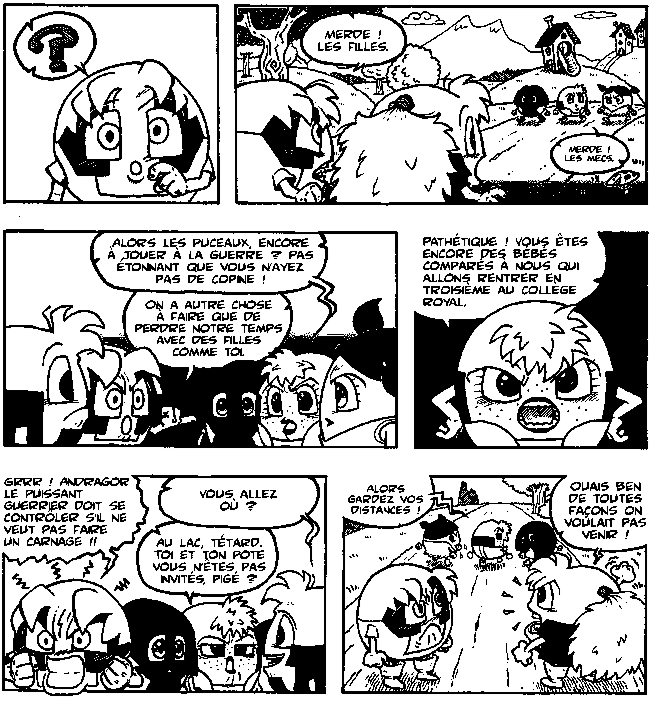
\includegraphics[trim= 0mm 0mm 0mm 0mm, clip, width=0.4\textwidth]{binary.png}}	\hspace{2em}
		\subfloat[Connected-component bounding boxes]{\label{fig:se:cc_bounding_box}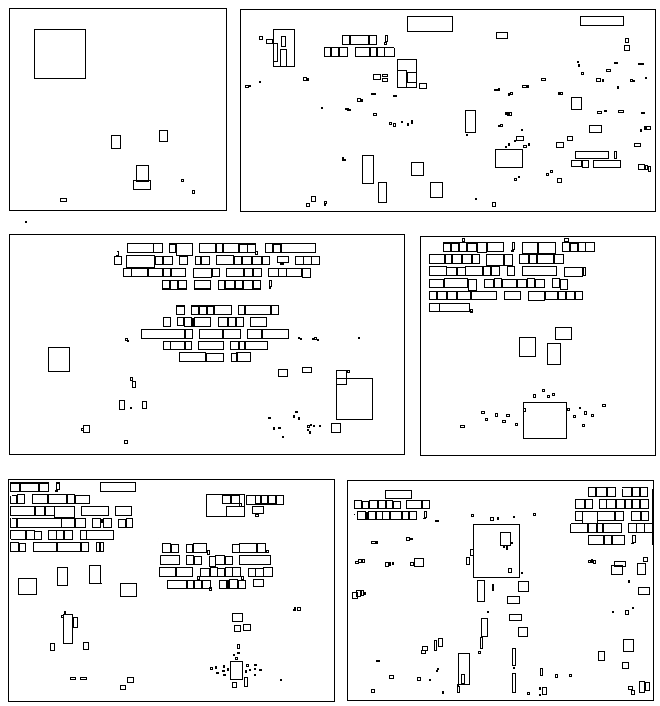
\includegraphics[trim= 0mm 0mm 0mm 0mm, clip, width=0.4\textwidth]{roi.png}}
		\\
		\subfloat[Panel cluster]{\label{fig:se:frame_unrecognized}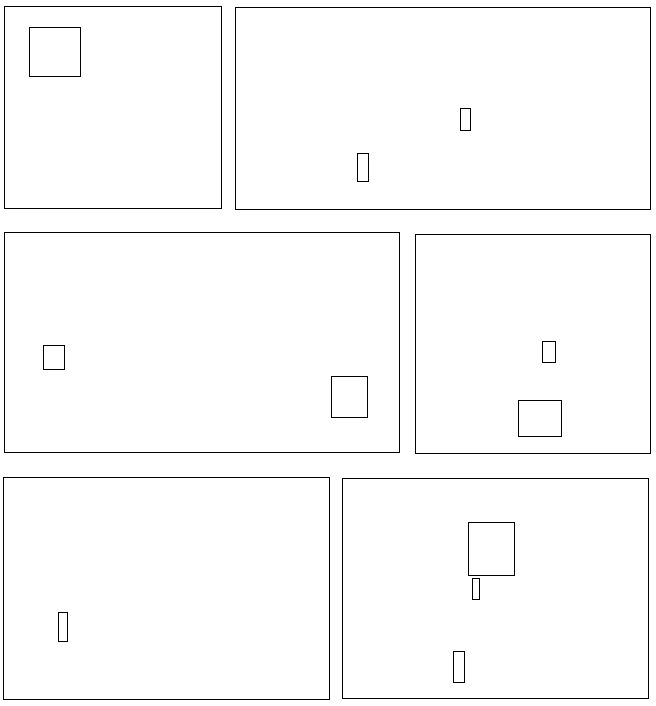
\includegraphics[trim= 1mm 0mm 0mm 0mm, clip, width=0.4\textwidth]{frame_unrecognized.png}}	\hspace{2em}
		\subfloat[Text cluster]{\label{fig:se:frame_cleaned}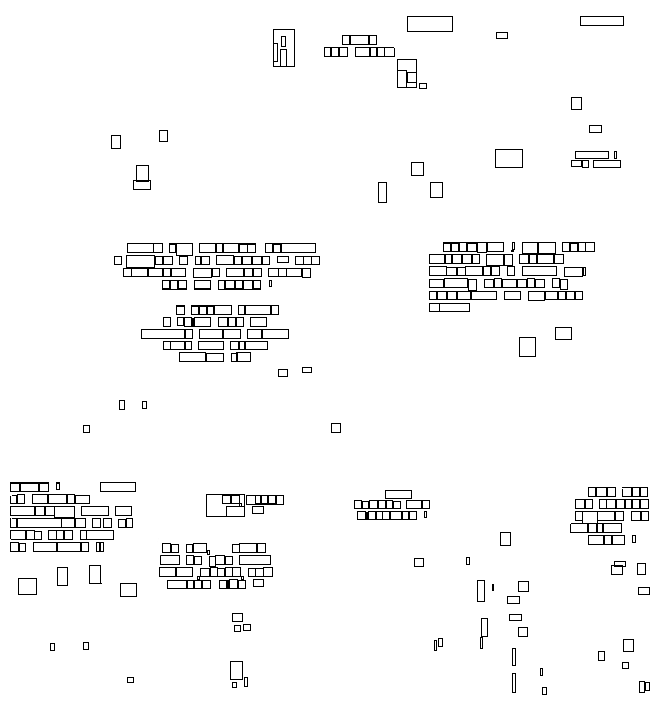
\includegraphics[trim= 1mm 0mm 0mm 0mm, clip, width=0.4\textwidth]{text.png}}
		  \caption[Panel extraction process]{Panel extraction process. Image credits:~\cite{Bubble09}.}
		  % \label{fig:se:binary_to_bounding_box}
	\end{figure}
	%%%%%%%%%%%%%%%%%%%%%%%%%%%%%%%%%%%%%%%%%%%%%%%%%%%

% paragraph process (end)

 % paragraph connected_component_extraction (end) 


\subsubsection{Clustering} % (fold)
\label{par:clustering}
By looking at the figure~\ref{fig:se:cc_bounding_box}, we can clearly see that the bounding boxes of the panel are bigger than the others.
Also, they include more regions than others.
Classifying those regions according to their size allows us to classify panel and text region at the same time while ignoring noise information.
Knowing the number of clusters facilitate the clustering, here 
% The classification of connected-component heights using k-means algorithm. 
%We define the set of component bounding boxes $R = \{R_1, R_2, ... , R_n\}$.
we set the number of clusters $k=3$ according to the domain knowledge of comics.
They aim to reflect the ``panel'' (the highest), the ``text'' (medium height) and the ``noise'' (few pixels height) as shown on figure~\ref{fig:se:histo_roi}.
One of the most popular clustering algorithm is k-means clustering method (Appendix~\ref{sub:ap:muli_threshold}).


This clustering is performed dynamically on each image which makes this method parameter-free (for a given number of clusters) and invariant to page format and resolution.
% Indeed, the height-based classification is not page size dependent unlike~\cite{Khoi11,Arai11}, and the number of pixels for each ROI is proportional to the page resolution (do not bias the classification).

	%%%%%%%%%%%%%%%%%%%%%%%%%%%%%%%%%%%%%%%%%%%%%%%%%%%
	\begin{figure}[!ht]	%trim=l b r t  width=0.5\textwidth, 
	  \centering
		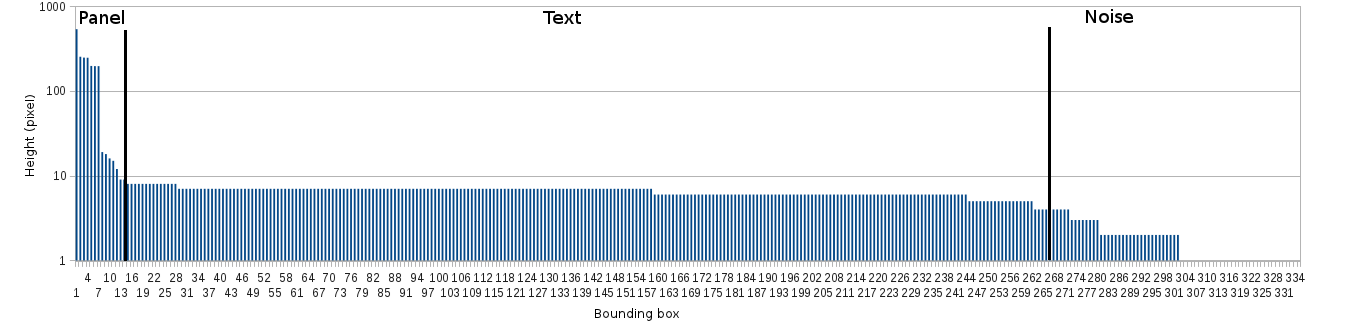
\includegraphics[trim= 5mm 0mm 10mm 0mm, clip,width=1.0\textwidth]{Histogram_en.png}
		\caption[Descendant histogram of the connected component bounding box heights]{Descendent histogram of the bounding boxes in figure~\ref{fig:se:cc_bounding_box}. Vertical black lines represent an example of three cluster limits labelled as ``panel'', ``text'' and ``noise''. Note that the lowest part of the ``panel'' cluster do not correspond to panel regions, we present how we pruned them in the next paragraph.}
		\label{fig:se:histo_roi}
	\end{figure}
	%%%%%%%%%%%%%%%%%%%%%%%%%%%%%%%%%%%%%%%%%%%%%%%%%%%

This method assumes that the image is highly contrasted and contains a high disparity between stroke sizes otherwise the binary segmentation or the clustering process may fail.

\subsubsection{Panel pruning} % (fold)
\label{par:se:pruning}

The results from the clustering operation can be pruned using domain knowledge.
The domain knowledge is given by the most followed conventions of comics design such as the panels that are usually juxtaposed and rarely included into each other~\ref{sub:intro:motivations}.
Note that the integration of the knowledge directly into the low level pruning process is restrictive for future processing that will have no chance to recover missing information.
Based on this assumption, we take out components which are included in other regions of the panel cluster.
% After the classification step, the second characteristic of panel is used in order to keep only the components that are not overlapped by others.
Given the set of component bounding boxes from the panel cluster $R = \{R_1, R_2, ... , R_n\}$, we filter out panel candidates that do not verify this relation $R_i\notin{R_j} \forall j, i \neq j$ (Figure \ref{fig:se:frame_candidates} and~\ref{fig:se:frame_cleaned}).

	%%%%%%%%%%%%%%%%%%%%%%%%%%%%%%%%%%%%%%%%%%%%%%%%%%%
	\begin{figure}	%trim=l b r t  width=0.5\textwidth, 
	  \centering
		\subfloat[Candidate panels]{\label{fig:se:frame_candidates}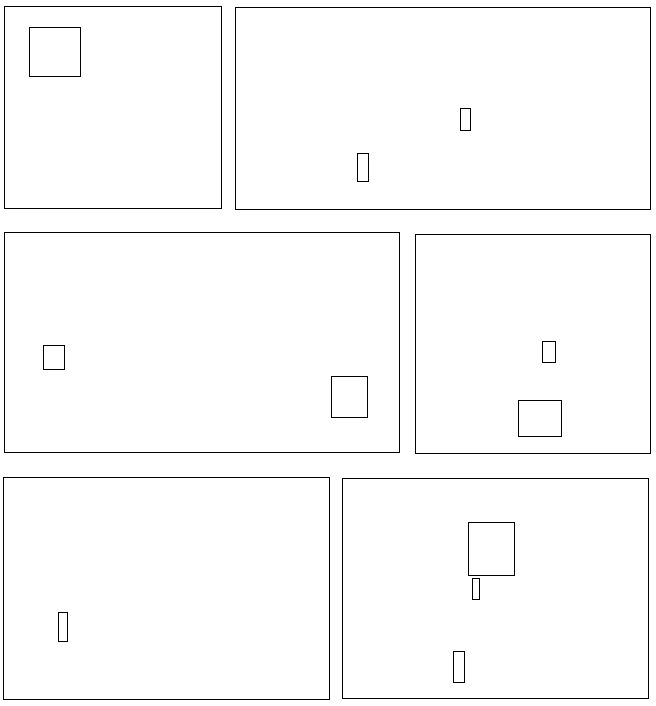
\includegraphics[trim= 1mm 0mm 0mm 0mm, clip, width=0.3\textwidth]{frame_unrecognized.png}}	\hspace{2em}
		\subfloat[Pruned panels]{\label{fig:se:frame_cleaned}
\includegraphics[trim= 1mm 0mm 0mm 0mm, clip, width=0.3\textwidth]{frame_cleaned.png}}
		  \caption[Topological pruning of panel bounding box extraction]{Topological pruning of panel bounding box extraction.}
		  %\label{fig:se:apl_1_0}
	\end{figure}
	%%%%%%%%%%%%%%%%%%%%%%%%%%%%%%%%%%%%%%%%%%%%%%%%%%%


\subsubsection{Letter to text line} % (fold)
\label{par:se:letter_to_line}
The gap between text component (e.g. letter or attached letters, word) and text lines can vary significantly.
In fact, handwriting generates a lot of artefacts such as alignment variations, mergers between letters and text lines.
We propose a simple method that handles the two first aforementioned artefacts considering the height and the neighbourhood of the connected-components.

Among all the connected-components (Figure~\ref{fig:se:cc_bounding_box}), we clearly see that the spatial organisation and the regular size are characteristics of text regions (regardless of the language).
We group text candidates into text lines according to alignment and ignore text candidate that can not be part of any text line.

Similarly to~\cite{Clavelli09,Li2013Comic}, we first search for the first letter (connected-component) of each text line and then attach the close and similar connected-components to the same text line.
A letter is considered first if it is positioned on the left, on the same horizontal line and if there is no intersection found with any other letters at a distance equal to the letter height.
Then the other letters on the right are added by checking their relative horizontal and vertical positions.
For this purpose, we defined two conditions that are auto-adaptive to each letter (Figure~\ref{fig:se:letter_position}):

\begin{itemize}
    \item The horizontal inter-letter distance $d$ should be smaller than the maximal height of the letters ($d<max(h_1,h_2)$);
    \item The vertical alignment is considered as correct if the vertical coordinate of the centre of the next letter $c_2$ passes through the first letter ($y_{min}(letter_1)>c_{2y}$ and $y_{max}(letter_1)>c_{2y}$);
\end{itemize}


%%%%%%%%%%%%%%%%%%%%%%%%%%%%%%%%%%%%%%%%%%%%%%%%%%%
\begin{figure}[h!]	%trim=l b r t  width=0.5\textwidth,
  \centering
	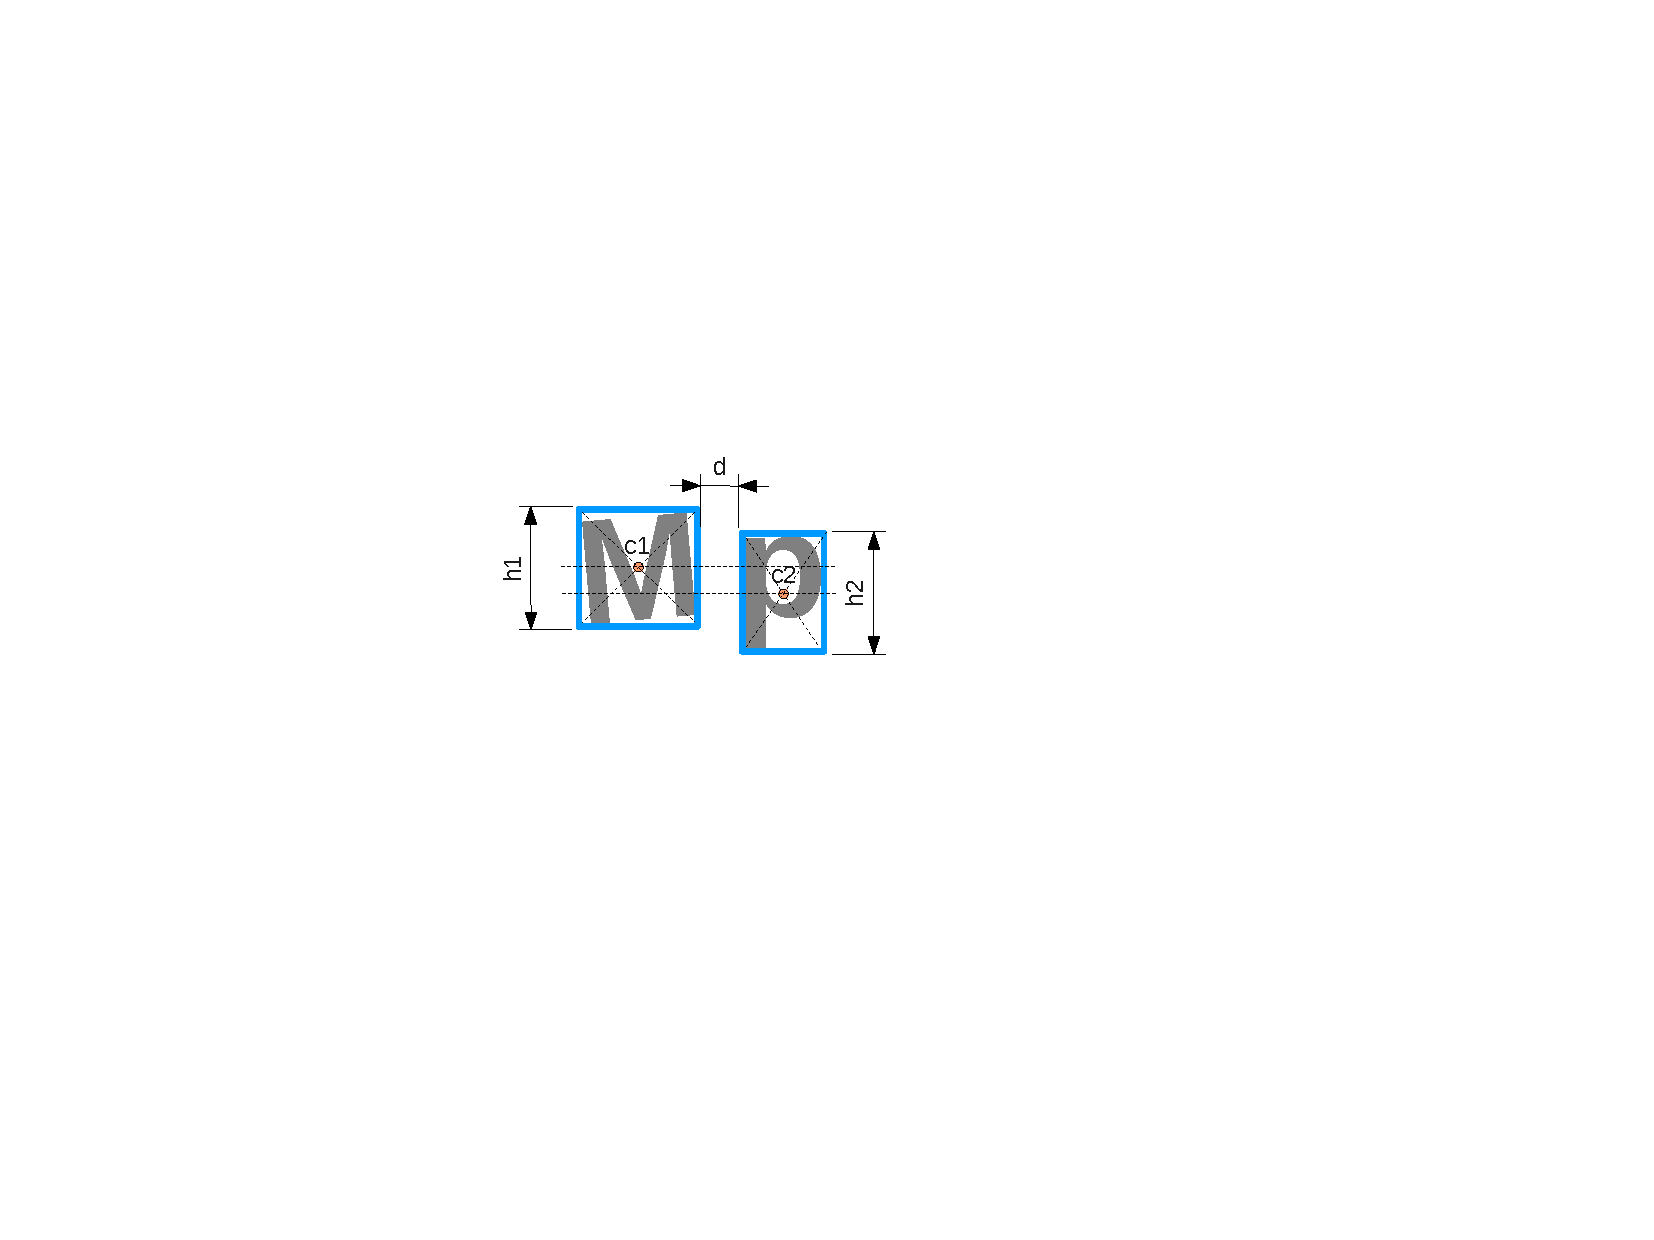
\includegraphics[trim= 0px 0px 0px 0px, clip, width=0.5\textwidth]{letter_position.pdf}
	\caption[Text component horizontal and vertical alignments]{Text component horizontal and vertical alignments. The two rectangles represent the bounding boxes and $c_1$ and $c_2$ their centres.}
	\label{fig:se:letter_position}
\end{figure}
%%%%%%%%%%%%%%%%%%%%%%%%%%%%%%%%%%%%%%%%%%%%%%%%%%%

The principle is similar to the one presented in~\cite{Clavelli09} but adapted to take into account the horizontal alignment of text lines.
Our method does not consider the letter width as we never know how many letters correspond to the CC.
This method can easily be used for vertical text (e.g. Japanese, Chinese and Korean) by switching horizontal and vertical measurements.
More text orientation can be handled using automatic multi-oriented touching character segmentation such as~\cite{Roy2009Multi}.




	% paragraph pruning (end)


% \paragraph{Text line construction} % (fold)
% \label{par:se:letter_to_line}


\subsubsection{Text line to paragraph} % (fold)
\label{par:text_line_grouping}

% As we are interested in localizing balloons from text, we post-process the results of the text line detection to group text lines into text area (paragraph), according to two rules.
We post-process the result of the text line detection to group text lines into text area (paragraph), according to two rules.
First, we require that the candidate text lines to group have similar heights (or width in case of vertical text) and second that the inter-line distance is smaller than the average text line height of the potential paragraph region (Figure~\ref{fig:se:line_to_paragraphs}).

	%%%%%%%%%%%%%%%%%%%%%%%%%%%%%%%%%%%%%%%%%%%%%%%%%%%
	\begin{figure}[h!]	%trim=l b r t  width=0.5\textwidth,
	  \centering
		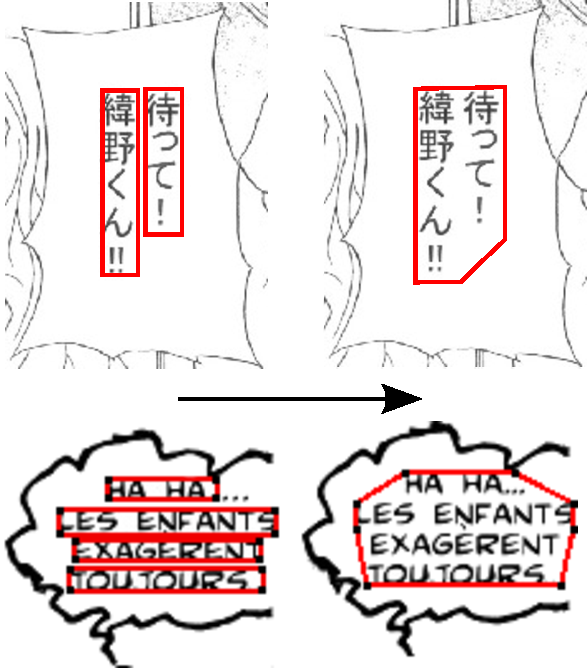
\includegraphics[trim= 0px 0px 0px 0px, clip, width=0.5\textwidth]{line_to_paragraphs.pdf}
		\caption[Text line to text paragraph conversion illustration]{Illustration of the text line to text paragraph conversion from left to right for vertical and horizontal text. Image credits:~\cite{Inoue08,Bubble09}}
		\label{fig:se:line_to_paragraphs}
	\end{figure}
	%%%%%%%%%%%%%%%%%%%%%%%%%%%%%%%%%%%%%%%%%%%%%%%%%%%

% paragraph text_line_grouping (end)

% paragraph classification (end)

% section panel_and_text (end)

\section{From text to balloon} % (fold)
\label{sec:se:from_text_to_balloon}
% In this section we detail a novel approach for closed and non-closed speech balloon localization in scanned comic book pages, an essential step towards a fully automatic comic book understanding. 
For comics content understanding, speech balloons are of significant interest since they offer the links between the textual content and the comic characters providing, in this way, information about the localization of the characters and the tone of speech. 
As mentioned in Section~\ref{sec:sota:balloon_segmentation}, speech balloons are the more frequent type of balloon in comics and are highly related to speech text regions.
In this section, we propose two approaches for balloon extraction based on text region location detection using the methods presented Section~\ref{sec:se:panel_and_text} or~\ref{sec:in:text_localisation_and_recognition}.
The first method defines as ``balloon'' the smallest connected-components that contain several text-like regions.
The second method groups text lines into paragraphs and initializes an active contour model (snake) on its outline.
From the initial position, the snake is pushed away from the text and attracted by surrounding edges at the same time in order to stick to any potential balloon stroke close by.
The main difference with the first approach is its ability to detect implicit or partially drawn balloons as well as the closed ones.

\subsection{Regular balloon extraction} % (fold)
\label{sub:se:regular_balloon_extraction}
Regular balloons are defined as closed balloons with a completely drawn contour unlike implicit contour discussed in the next Section~\ref{sub:se:implicit_balloon_extraction}.
Closed balloons are easily extractable using blobs detection method similarly to the panel and text extraction presented above.
The main difference lies in their dominant colour which is generally white and implies to extract white connected-components instead of black ones as for panels and text.
One particularity of text inside balloons is its vertical and/or horizontal alignment in the balloon (Figure~\ref{fig:se:text_in_balloon}).
We propose to use this characteristic to compute a confidence value to each connected-component that includes one or more text regions.

	%%%%%%%%%%%%%%%%%%%%%%%%%%%%%%%%%%%%%%%%%%%%%%%%%%%
	\begin{figure}[h!]	%trim=l b r t  width=0.5\textwidth,
	  \centering
		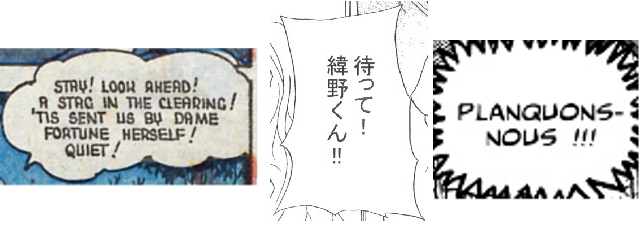
\includegraphics[trim= 0px 0px 0px 0px, clip, width=0.75\textwidth]{text_in_balloon.png}
		\caption[Text positions in speech balloons]{Example of text positions in speech balloons. Image credits~\cite{McCall46,Inoue08,Bubble09}.}
		\label{fig:se:text_in_balloon}
	\end{figure}
	%%%%%%%%%%%%%%%%%%%%%%%%%%%%%%%%%%%%%%%%%%%%%%%%%%%

% The alignment confidence can be used in a later stage to classify balloon and non regions.
\subsubsection{Blob extraction} % (fold)
\label{par:blob_extraction}

A typical ``closed'' balloon is surrounded by a black stroke that defined a white region (blob) inside it, with holes created by the presence of text letters.
We propose to make a binary segmentation of the comics image and then use connected-component labelling method to extract white blobs (Figure~\ref{fig:se:closed_balloon}).
We assume that closed balloons are surrounded by a stroke with similar darkness and stroke-width from one balloon to another in a given scanned image.
In this context, global segmentation methods are appropriate because the optimal threshold selection is similar for all balloon regions.
% Binary segmentation (binarisation) aims to separate the page background (clear region) from its content (dark strokes).
We use Otsu's threshold selection method to find the optimal threshold (Appendix~\ref{sub:ap:bi_threshold}).
%Here, we do not use a local segmentation approach because it increases the chances to split the strokes that compose balloon contours by choosing a too low of too high threshold value.

	%%%%%%%%%%%%%%%%%%%%%%%%%%%%%%%%%%%%%%%%%%%%%%%%%%%
	\begin{figure}[h!]	%trim=l b r t  width=0.5\textwidth,
	  \centering
		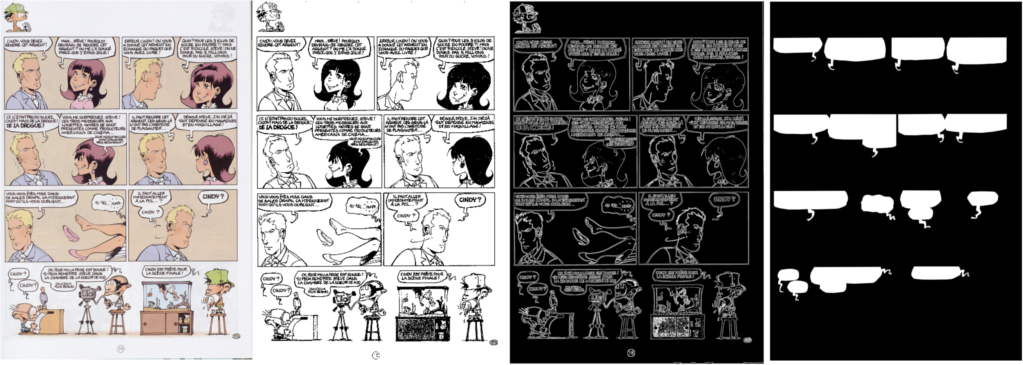
\includegraphics[trim= 0px 0px 0px 0px, clip, width=0.75\textwidth]{closed_balloon_process.png}
		\caption[Sequential balloon extraction process illustration]{Balloon extraction process. Original image, binary segmentation, contour detection (connected components) and result mask from left to right. Image credits:~\cite{Midam01}. }
		\label{fig:se:closed_balloon}
	\end{figure}
	%%%%%%%%%%%%%%%%%%%%%%%%%%%%%%%%%%%%%%%%%%%%%%%%%%%


% paragraph blob_extraction (end)


\subsubsection{Balloon extraction} % (fold)
\label{par:balloon_extraction}

For each extracted blob that includes a text paragraph (Section~\ref{par:text_line_grouping}), we compute the difference of alignment on the horizontal $d_x$ and the vertical $d_y$ axis between the balloon barycentre $c_1$ and the text paragraph barycentre $c_2$ (Figure~\ref{fig:se:align_diff}).
We use the difference of alignment as a confidence value $C_{balloon}$ for balloon and non-balloon classification (\ch{chap:experimentations}).

	%%%%%%%%%%%%%%%%%%%%%%%%%%%%%%%%%%%%%%%%%%%%%%%%%%%
	\begin{figure}[h!]	%trim=l b r t  width=0.5\textwidth,
	  \centering
		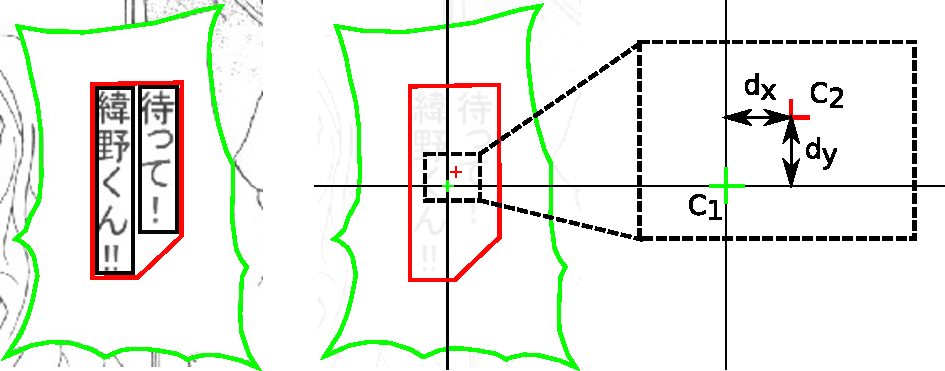
\includegraphics[trim= 140px 0px 0px 0px, clip, width=0.5\textwidth]{text_balloon_alignment.pdf}
		\caption[Illustration of the vertical and horizontal alignment differences between balloon and text region barycentre]{Vertical $d_y$ and horizontal $d_x$ alignment differences between balloon barycentre $c_1$ and text region barycentre $c_2$.}
		\label{fig:se:align_diff}
	\end{figure}
	%%%%%%%%%%%%%%%%%%%%%%%%%%%%%%%%%%%%%%%%%%%%%%%%%%%

Both differences $d_x$ and $d_y$ are normalized between zero and one as a percentage of the balloon width $B_{width}$ and height $B_{height}$ respectively.
The average of the vertical and horizontal alignments gives a confidence value for each balloon candidate (Formula~\ref{eq:se:balloon_confidence_value}).


\begin{equation}
	\label{eq:se:balloon_confidence_value}
	C_{balloon} = 1 - \frac{1}{2} *  \bigg( \frac{d_x}{B_{width}} + \frac{d_y}{B_{height}} \bigg)
\end{equation}

If the sum of differences of alignment is higher than the balloon size ($d_x > B_{width}$ and $d_y > B_{height}$) then $C_{balloon}$ becomes negative which is considered as $C_{balloon}=0$.
An alternative could be to compare the axis of the main moment of inertia of text and balloon regions.



% paragraph balloon_extraction (end)


% subsection regular_balloon_extraction (end)

\subsection{Implicit balloon extraction} % (fold)
\label{sub:se:implicit_balloon_extraction}

Balloon contour is not always completely drawn, it may be implied by contextual information such as contrast difference or other surrounding elements (Figure~\ref{fig:se:balloon_examples}c).
In most of the cases, the location of text is a good clue to guess where the speech balloons are.
The problem of speech balloon outline detection can therefore be posed as the fitting of a closed contour around text areas, with the distinctiveness that the outline might not be explicitly defined in the image.
For the examples given in Figure~\ref{fig:se:balloon_examples}, this would be a smooth contour with relatively constant curvature (Figure~\ref{fig:se:balloon_examples}a), an irregular one with high local curvature (Figure~\ref{fig:se:balloon_examples}b), and an implicit one with missing parts (Figure~\ref{fig:se:balloon_examples}c).
Through these observations, we can see how important the domain knowledge is, in the global interpretation process.

	%%%%%%%%%%%%%%%%%%%%%%%%%%%%%%%%%%%%%%%%%%%%%%%%%%%
	\begin{figure}[!ht]%trim=l b r t  width=0.5\textwidth,
	\begin{center}
	  \begin{tabular}{ccc}
	  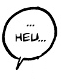
\includegraphics[trim= 0px 2px 0mm 0mm, clip, width=0.13\textwidth]{round_balloon.png}&
	  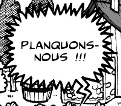
\includegraphics[trim= 0mm 0mm 0mm 0mm, clip, width=0.17\textwidth]{peaked_balloon.png}&
	  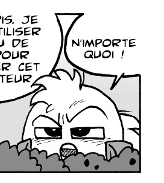
\includegraphics[trim= 15px 7mm 5px 0mm, clip, width=0.145\textwidth]{open_balloon.png} \\ 
	  \footnotesize a) Smooth	& \footnotesize b) Irregular & \footnotesize c) Implicit
	  \end{tabular}
	\caption[Speech balloon contour types]{Example of speech balloons with different contour types. Image credits~\cite{Bubble09}.}
	\label{fig:se:balloon_examples}
	\end{center}
	\end{figure}	
	%%%%%%%%%%%%%%%%%%%%%%%%%%%%%%%%%%%%%%%%%%%%%%%%%%%

Observing the heterogeneity of balloons, and considering the difficulty to manage ``open'' or ``implicit'' balloons, it appears necessary to use a dynamic and adaptive outline detection algorithm.
Active contours appear to be suitable to the problem.
The active contour framework was developed for delineating an object outline in an image.
The algorithm attempts to minimize the energy associated to the current contour, defined as the sum of an internal and an external energy term (Appendix~\ref{sub:ap:contour_based}). 
In this section we propose two adaptations of the active contour theory to the domain of comic balloon detection.
Specifically, we handle the case of balloons with missing parts or implicit contours, while we adopt a two-step approach to fit irregular outline types such as peak and cloud type balloons. 
To achieve this, we propose new energy terms making use of domain knowledge.


% %------------------------------------------------------------------------
% \subsubsection{Active contours TODO: move to SOTA}
% \label{sec:se:active_contour}

% The active contour~\cite{Kass1988} model is a deformable model, also known as snake, corresponding to a curve $\mathbf{v}(s)=[x(s),y(s)], s \in [0,1]$, that moves through the spatial domain of an image to minimize the energy functional (equation~\ref{eq:se:energy1}).

% \begin{equation}\label{eq:se:energy1}
%   E = \int_0^1 \! \frac{1}{2} \left( \alpha \left|\mathbf{v}'(s) \right|^2 + \beta \left| \mathbf{v}''(s) \right|^2 \right) + E_{ext}(\mathbf{v}(s))ds\\
% \end{equation}
% where $\alpha$ and $\beta$ are weighting parameters that respectively control the snake's tension and rigidity, and $\mathbf{v}'$ and $\mathbf{v}''$ denote the first and second derivatives of $\mathbf{v}(s)$ with respect to $s$. This functional energy is also called $E_{int}$ for internal energy.
% The external energy function $E_{ext}$ is computed from the image so that it takes on its smaller values at the features of interest, such as boundaries~\cite{Xu1998}.
% %It was initially designed to localize nearby edges accurately by using both internal and external energies (see eq.~\ref{eq:se:energy1}). 
% %The external energy function $E_{ext}$ aim to attract the snake to the feature of interest (e.g. line, edge, corner), it is the image force. 
% One of the proposed energy functions by Kass~\cite{Kass1988} is equation~\ref{eq:se:edge} which attracts the contour to edges with large image gradients. 
% \begin{equation}\label{eq:se:edge}
%   E_{ext} = -|\nabla \mathbf{I}(x,y)^2|
% \end{equation}

We adapt the active contour framework to the domain of comics to detect speech balloons given a prior detection of text regions, introducing new energy terms based on domain knowledge about the relationship between text and balloons.
For the discussion below, we assume that text has been already detected in the image (Section~\ref{sec:se:panel_and_text} and~\ref{sec:in:text_localisation_and_recognition}).% and we use the method of \cite{Rigaud2013VISAPP} for text detection.

The introduction of statistical shape knowledge has already been studied in the literature but can not be applied here because of the lack of knowledge about the contour shape to detect and complex background~\cite{Cremers2002}.
The original active contour model proposed by Kass~\cite{Kass1988} defines a energy function composed by internal $E_{int}$ and external $E_{ext}$ forces that make the initial contour shrinks to the object boundaries (Appendix~\ref{sub:ap:contour_based}).
As we assume that text is included inside balloons, we need to inflate instead of shrink the initial contour in order to retrieve or approximate the balloon boundary.
For this purpose, we introduce a new energy term denoted $E_{text}$ that conveys information about the relative placement of the balloon outline and the enclosed text (Equation~\ref{eq:se:energy2}).

\begin{equation}\label{eq:se:energy2}
  E = E_{int} + E_{ext} + E_{text}\\
\end{equation}

\subsubsection{External energy}
\label{sec:se:external_energie}
%The external energy $E_{ext}$ encourage curve onto image structures (e.g. edges, line, corner).

We consider edges as features of interest because we expect the speech balloon to be delimited by strong edges, at least partially.
Here we perform edge detection using the well-known Sobel operator (Figure~\ref{fig:se:distance_transform}).
According to the review of state of the art methods appropriate for implicit balloon detection (Section~\ref{sec:sota:balloon_segmentation}), active contour models are good choices.
Appendix~\ref{sub:ap:contour_based} gives the basic concepts of the original approach proposed by Kass~\cite{Kass1988}.
In this approach, the definition of the external energy is appropriate for natural scene images with smooth gradients but not for stroke-based images such as comics that comprise uniform coloured regions (flats) with strong edges (strokes).
In our case, we require that edges attract the snake from relatively far away (distances where the original edge gradient has already dropped to zero).
The method of Xu~\cite{Xu1998} would be appropriate here, although we have decided to use the equivalent distance transform of the edge image instead for computational efficiency reasons.
We therefore define the external energy function as:

\begin{equation}\label{eq:se:energy3}
  E_{ext} = \gamma \min A(i,j) = \gamma \min  \sqrt{(x_i-x_j)^2+(y_i-y_j)^2}\\
\end{equation}
where $E_{ext}$ is the minimum Euclidean distance ($A$) between a point $i$ and the nearest edge point $j$, $\gamma$ is a weighting parameter.

Since it is not desirable for edges corresponding to text to attract the snake, any edges that fall within the text regions are removed before computing the distance transform and do not contribute to the external energy.
	
	%%%%%%%%%%%%%%%%%%%%%%%%%%%%%%%%%%%%%%%%%%%%%%%%%%%
	\begin{figure}[!ht]	%trim=l b r t  width=0.5\textwidth,
	  \centering
		\fbox{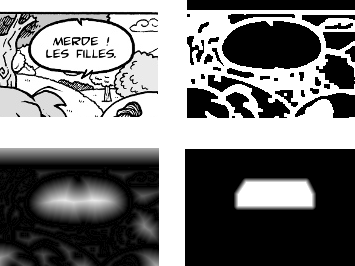
\includegraphics[trim = 0mm 0mm 7mm 0mm, clip, width=230px]{edge_dist_trans.png}}
		\caption[Active contour energies for open balloon extraction]{Example of original image (top left) and its corresponding non-text edge detection (top right), $E_{ext}$ energy (bottom-left) and $E_{text}$ energy (bottom-right). In the bottom part, white corresponds to high energy. Image credits:~\cite{Bubble09}. }
		\label{fig:se:distance_transform}
	\end{figure}
	%%%%%%%%%%%%%%%%%%%%%%%%%%%%%%%%%%%%%%%%%%%%%%%%%%%

\subsubsection{Internal energy}
We use the original definition of the internal energy (Equation~\ref{eq:se:energy1}) which can by decomposed in two energy terms: $E_{cont} = \left|\mathbf{v}'(s) \right|^2$ and $E_{curv}=\left| \mathbf{v}''(s) \right|^2$.
%It is composed of a continuity and a curvature energies: $E_{internal} = \alpha E_{cont} + \beta E_{curv}$ as defined in eq.~\ref{eq:se:energy3}. The coefficients $\alpha$ and $\beta$ give more or less importance to one energy or another.
% 
% \begin{equation}\label{eq:se:energy3}
%   E_{internal} = \left( \alpha(s)  \left|\frac{d\bar{v}}{ds}(s) \right|^2 + \beta(s) \left| \frac{d^2\bar{v}}{ds^2}(s) \right|^2 \right) /2
% \end{equation}

The energy $E_{cont}$ forces the contour to be continuous by keeping points at equal distance, spreading them equally along the snake according to the average inter-point distance of the contour.
It becomes small when the distance between consecutive points is close to the average (Equation~\ref{eq:se:cont}).

\begin{equation}\label{eq:se:cont}
 E_{cont} = \alpha \Big|\bar{d} - \sqrt{(x_i - x_{i-1} )^2 + (y_i - y_{i-1} )^2}\Big|
\end{equation}
where $\bar{d}$ is the average distance between two consecutive points $i$ and $j$ of the snake and $\alpha$ is a weighting parameter.

The energy $E_{curv}$ enforces smoothness and avoids oscillations of the snake by penalizing high contour curvatures (minimizing the second derivative).
It becomes small when the angle between three consecutive points is close to zero (Equation~\ref{eq:se:curv}).
% Note, this energy itself makes the snake deflate and converge to a line or a point.

\begin{equation}\label{eq:se:curv}
  %E_{curv} = \beta | p_{i-1} - 2 * p_i + p_{i+1} |^2
  E_{curv} = \beta \left( (x_{i-1} - 2x_{i} + x_{i+1})^2 + (y_{i-1} - 2y_{i} + y_{i+1})^2 \right)
\end{equation}
where $i$ is a point of the snake and $\beta$ a weighting parameter.

%The distance $h1$ is an a priori distance between the text and its balloon. % for positioning the snake when there is a lake of external energy at low resolution detection.
%The distance $h2$ is the difference between the outer and the inner distance

\subsubsection{Text energy}
\label{sec:se:text_energie}

The text energy $E_{text}$ conveys domain specific knowledge about the relative locations of text areas and their associated balloon contours in this domain.
It is necessary to consider the lack of explicit information in the cases of implicit balloons, where parts of the outline are missing.
The $E_{text}$ energy aims at pushing the snake outwards toward the most likely balloon localization, given the position of the text area.
This energy term has two effects.
First, it acts collaboratively to the external energy, by moving the snake towards non-text edges (hopefully corresponding to the balloon outline).
Second, in the case of implied contours where no explicit edge exists (the external energy term is not informative), $E_{text}$ assists the algorithm to converge to an approximate contour position based on prior knowledge on the expected localization given the corresponding text area.
We define the text energy term at localization $i$ of the image as follows:

\begin{equation}\label{eq:se:know}
E_{text} = \begin{cases} \kappa \frac{N}{min_{j \in T} A(i,j)} & \mbox{if } A(i,j) > 0 \\ \kappa N & \mbox{else} \end{cases}
\end{equation}
where $j$ is a pixel in the text area $T$, $N$ is an experimentally defined constant expressing the expected distance in pixel between the text area and the corresponding balloon boundary and $\kappa$ is a weighting parameter that controls the contribution of $E_{text}$ with respect to the other energy terms in Equation~\ref{eq:se:energy2}. Note when $i$ is on the border of $T$, the distance $A(i,j)$ is equal zero and the energy becomes maximal as if it was inside $T$.


\subsubsection{Proposed method}
\label{sec:proposed_method}

In this section we detail how to localize speech balloons using active contours based on the definitions given above. 
First we generate the static external energy map $E_{ext}$ for the whole image and then for each text area we compute the $E_{text}$ energy.
The internal energy $E_{int}$ is calculated for each point of the snake before each iteration.
We iteratively examine each point of the snake in a clockwise fashion and move it within a neighbourhood region of size $M$ in order to minimize Equation~\ref{eq:se:energy2}.
This operation is repeated until no point moves in one turn (Algorithm~\ref{al:be:method}).
Detecting the implicit parts of the balloons is quite challenging as we aim at detecting something which is not in the image, by interpolating contextual information (other printed part of the balloon).
We propose a two step approach to test if the information is present or not before trying to extract it precisely.
It is similar to our visual system or other computer-based object detection approaches which are able to decide if an object is present or not before finding its exact shape (coarse to fine).
First, we perform a coarse balloon contour position approximation (low resolution) using a quite rigid snake model.
Then we fit the contour better to have a fine extraction of the balloon contour (high resolution) using the same algorithm and tuning the energy weighting parameters in a way to relax the snake (increase flexibility).
The idea is to start a high resolution contour detection only when the active contour is positioned close to the contour.
Otherwise, if we start the balloon detection using a too flexible snake, it might be attracted by forces that do not come from a balloon edge before reaching the contour position (printed or suggested).

% TODO: remove high resolution step???
%, especially for non-smooth boundaries.% High resolution contour shape fitting - aiming to 
 %\item Contour classification [NOVELTY? SHAPE COMPOSED BY DIFFERENT PART OF SHAPE]

\begin{algorithm}
\caption{Open balloon detection loop}
\label{al:be:method}
\begin{algorithmic}
%\REQUIRE $n \geq 0 \vee x \neq 0$
%\ENSURE $y = x^n$
%\STATE $y \leftarrow 1$
\STATE{compute $E_{ext}$ energy}
\FOR{each text area}
  \STATE compute $E_{text}$ energy
  \STATE active contour initialization
  \STATE stop = False
  \WHILE{stop = False}%\STATE{DO}
    \STATE $n = 0$
    \FOR{each points of the snake}
      \STATE examine neighbourhood position energies
      \IF{one position reduce the current energy}
		\STATE move point to this position
		\STATE $n=n+1$
      \ENDIF
    \ENDFOR
    % \STATE // If not points have been moved then stop
    \IF{$n = 0$}
    	\STATE{stop = True}
    \ENDIF
  \ENDWHILE% <--- use \doWhile for the "while" at the end %\While{$n > 0$}
\ENDFOR
\end{algorithmic}
\end{algorithm}

\paragraph{Active contour initialisation}
\label{sec:se:cont_init}

The active contour is initialized on the outline of the text paragraph region.
This corresponds to the convex hull of all the text lines that are included in the balloon (Figure~\ref{fig:se:paragraphs}b).
Note that the convex hull of the text area also corresponds to the $E_{text}$ maximal value border (Figure~\ref{fig:se:distance_transform}).
%At this point, the $E_{text}$ has to be the strongest in eq.~\ref{eq:se:energy2} in order to ``push'' away the snake from the text area and then facilitate its attraction by $E_{ext}$ (non text edges).
%Another possible initialization strategy could be to use the smaller ellipse circumscribing the text area.% This has been experimented section~\ref{sec:experiments}.

%Note, in case of wrong initialization, the external energy allow the snake to inflate deflate in the case of the snake initialization is outside the balloon. Gradients that are inside the initial curve repulsed the contour (considered as text areas).


%\subsubsection{Number of points}
The initial number of points impacts the way that the snake moves and the precision of the final detection.
During the first low resolution localization step, we perform a spaced equipartition of the points (Figure~\ref{fig:se:paragraphs}c) to quickly localize the global shape avoiding unnecessary stops on image details.
In the subsequent high resolution fitting stage, we add more intermediate points to fit the exact shape more precisely.
% with an inter-points distance fixed to half line height

%%%%%%%%%%%%%%%%%%%%%%%%%%%%%%%%%%%%%%%%%%%%%%%%%%%
	\begin{figure}[!ht]%trim=l b r t  width=0.5\textwidth,
	\begin{center}
	  \begin{tabular}{ccc}
	  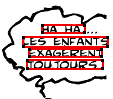
\includegraphics[trim= 0mm 0mm 0mm 0mm, clip, width=0.20\textwidth]{group_lines.png}&
	  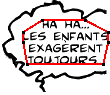
\includegraphics[trim= 0mm 0mm 0mm 0mm, clip, width=0.20\textwidth]{convex_hull.png}&
	  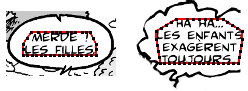
\includegraphics[trim= 48mm 0mm 0mm 0mm, clip, width=0.20\textwidth]{snake_init.png} \\ 
	  \footnotesize a) Group of text lines	& \footnotesize b) Text area convex hull 	& \footnotesize c) Snake initialization 
	  \end{tabular}
	\caption[Active contour initialization based on text region convex hull]{Active contour initialization based on text region convex hull. Image credits:~\cite{Bubble09}.}
		\label{fig:se:paragraphs}
	\end{center}
	\end{figure}	
	%%%%%%%%%%%%%%%%%%%%%%%%%%%%%%%%%%%%%%%%%%%%%%%%%%%


%We initialize the active contour of $N$ points on the paragraph shape (group of lines) figure~\ref{fig:se:paragraphs} and then we make it grow until it hits edges.
%We define a paragraph as a group of text lines spoken by the same speaker and with no interruptions (e.g. time break, interaction, other person talk). These group of lines are written close to each other by convention . We labelize two consecutive lines as part of the same paragraph if there is no enough space for an other line similar in height between them.

\paragraph{Low resolution contour fitting}
Following a two stage process, we first aim to obtain a rough localization of the balloons by fitting a coarse contour using a few contour points during the initialization.
The idea is to progressively push the snake away from the text area and towards the balloon boundary giving an increased weight to both the $E_{ext}$ and $E_{text}$ energy terms.
If the balloon has an explicit boundary then $E_{ext}$ will attract the snake to it.
If there is no explicit contour close enough to attract the snake then the $E_{text}$ term will push the snake to the suggested position of the balloon contour.
Also the internal energies are important at this stage to maintain a certain rigidity of the snake.
%The and low external energy parameter $\gamma$, a large internal curvature energy parameter $\beta$ and a large knowledge energy parameter $\eta$ (Fig.~\ref{fig:se:multiscale01}). 
At the end of this step, we obtain a coarse description of the balloon contours which can be sufficient for localisation purposes but not for balloon type classification for instance (Figure~\ref{fig:se:mono_res_det}). 

	%%%%%%%%%%%%%%%%%%%%%%%%%% which cadescription be enough for  contourlocalisation purposes but not for balloon type classification based on contour type for instance%%%%%%%%%%%%%%%%%%%%%%%%%
	\begin{figure}[!ht]	%trim=l b r t  width=0.5\textwidth,
	  \centering
		% \fbox{
		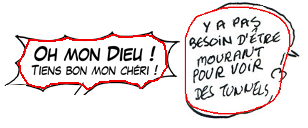
\includegraphics[trim = 0mm 3mm 0mm 1mm, clip, width=220px]{mono_res_det.png}
		% }
		\caption[Examples of low resolution contour detection for balloon extraction]{Example of low resolution balloon contour detection (red line) for irregular closed (top) and smooth open (bottom) speech balloons. Image credits:~\cite{EtPisTaf12,Montaine11}.}
		\label{fig:se:mono_res_det}
	\end{figure}
	%%%%%%%%%%%%%%%%%%%%%%%%%%%%%%%%%%%%%%%%%%%%%%%%%%%

% \subsection{Candidate point selection}
% {\bf SECTION REMOVED because we don't know yet how to efficiently select the point and because multi-resolution method already improves results without using candidate point selection. We can mention it in the prospects.}

%The candidate point selection aim to determine if the snake segments between points can be more detailed or not (e.g. detection of peak, circle, tail). Figure~\ref{fig:se:multiscale01} shown two categories of points, those who has been attracted and stopped by edge (part of the real contour) and the others (part of the suggested contour). At this point we can see that adding more points on the real contour parts and relaxing the internal energies could improve the contour detection. This a true but then all the contour will be affected and we could degrade the suggested contour detection part if it is a non closed contour. Therefore we add new points only between those stopped by edge because we can not get more detail about suggested parts of the contour and we could even loose the low resolution detection information.
%We consider as ``stopped'' the points that are common with the ``text less'' edge map (left part of fig.~\ref{fig:se:distance_transform}).
 %An example of candidate points is on figure~\ref{fig:se:multiscale01} and~\ref{fig:se:multiscale02}). We keep those new generated points only if they hit and edge before the snake stabilize again (only if they improve the contour detection). The aim is to get a higher resolution contour detection only where there is a contour drawn. If no contour (non closed balloon case) then we keep the appropriate shape from low resolution detection.


\paragraph{High resolution contour fitting}
Figure~\ref{fig:se:mono_res_det} shows that the global shape of the top balloon has already been retrieved, even for the implicit contour parts.
% , although it is can not be considered as a perfect balloon extraction as a lot of contour variation details are missing.
% As we can see on the bottom part of the balloon, the snake was not able to fit precisely balloon outline, for instance peaky and tail regions are not well segmented.
The aim of the high resolution fitting process is to attract the snake to the balloon contour details where they are drawn and keep the implicit contour position found by the low resolution process elsewhere.
To achieve a fine detection, we increase the resolution of the snake by adding new points between to the snake, changing the weighting parameters of the energy function and go through a second fitting process using the same Algorithm~\ref{al:be:method}.
At this stage, we relax the $E_{curv}$ energy to make the snake fit thinner parts of the image and we set $E_{cont}$ strong enough to keep a regular inter-point distance all over the contour.
Also, we reduce the $E_{text}$ energy weight because at this step, the snake is already far from text and this term is not informative any more.
%to give more importance to the image energy than the prior knowledge. %is reduced because  external  avoid point  is closer to the final contour and do not need the $E_{know}$ energy start to minimize we reduced the inter-points distance, we also increase the external energy parameter $\gamma$ to make the snake more attractable by image edge, decrease the internal curvature energy parameter $\beta$ to allow more flexible contour fitting and decrease the knowledge energy parameter $\eta$ because the contour is now far from the text. 
This new configuration allows the snake to fit more precisely to the balloon contour as shown in Figure~\ref{fig:se:hd_contour} (to compare with Figure~\ref{fig:se:mono_res_det}).

%{\bf TO ADD IF RESULTS CONFIRMS: we consider external energy map based from edge detection only (no distance transform any more)?}

	%%%%%%%%%%%%%%%%%%%%%%%%%%%%%%%%%%%%%%%%%%%%%%%%%%%
	\begin{figure}[!ht]	%trim=l b r t  width=0.5\textwidth,
	  \centering
		% \fbox{
		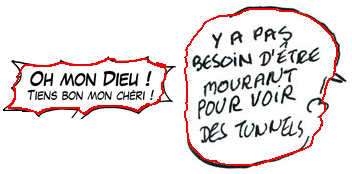
\includegraphics[trim = 0mm 2mm 0mm 1mm, clip, width=180px]{multi_res_det.png}
		% }
		\caption[Examples of high resolution contour detection for balloon extraction]{Examples of high resolution contour detection (red line) for closed (left) and open (right) balloons.}
		\label{fig:se:hd_contour}
	\end{figure}
	%%%%%%%%%%%%%%%%%%%%%%%%%%%%%%%%%%%%%%%%%%%%%%%%%%%

% subsection implicit_balloon_extraction (end)

% section from_text_to_balloon_ (end)

\section{From balloon to tail} % (fold)
\label{sec:se:from_balloon_to_tail}

% \modif{TODO: JMO: introduire ici toutes les difficultés liés aux queues pour ne pas les découvrir tout au long de la présentation de la méthode. Commencer par présenter le problème, ses difficultés (e.g. diversité des queues, niveau de représentativité, la difficulté à les analyser et éventuellement rappeler la litterature existante et le spectre couvert ou non de la litterature), ses enjeux, son existance dans la littérature. Ensuite dérouler les méthodes comme cela est fait. Valable pour toute les autres méthodes aussi :)}

%Balloon tails tell the reader the relationships between a set of textual or graphic elements contained in the speech balloons and the comics characters [REF???].
Tails are part of the balloon contour, they make the visual relation between the two most important elements in comics: balloons and comic characters (Section~\ref{sec:sota:balloon_segmentation}).
Speech balloons indicate dialogue using tails pointing at their respective speakers~\cite{Varnum2007Language}.
From our knowledge, detection has not been studied before even-through it is key information for comics understanding.
They are represented by a discontinuity on balloon contour (Figure~\ref{fig:se:tail_types}).

    %%%%%%%%%%%%%%%%%%%%%%%%%%%%%%%%%%%%%%%%%%%%%%%%%%%%%%%%
    \begin{figure}[h]%trim=l b r t  width=0.5\textwidth,  
      \centering
      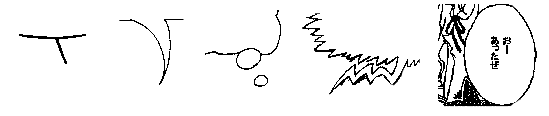
\includegraphics[trim= 0px 0px 0mm 0mm, clip, width=0.75\textwidth]{tail_types.png}
    \caption[Examples of type of speech balloon tails]{Examples of type of speech balloon tails. From left to right: stroke, comma, circle, zigzag, absent.}
    \label{fig:se:tail_types}
    \end{figure}
    %%%%%%%%%%%%%%%%%%%%%%%%%%%%%%%%%%%%%%%%%%%%%%%%%%%%%%%%

The first interesting information to extract is: where the tail is \emph{connected} to the balloon and the position of its tip (extremity).
From these two information we can compute a first direction and try to find the character to which it is related to in a post processing.
Here comes the main difficulties, the tail may change direction several times from its origin to the tip, only the last part of the tail indicates the direction of the speaking character.
Moreover, depending on the method used for extracting balloons, the tail tip position can be predicted in the background region or on the balloon boundary (more accurate) which may give a different direction at the end (Figure~\ref{fig:se:tail_examples}).


    %%%%%%%%%%%%%%%%%%%%%%%%%%%%%%%%%%%%%%%%%%%%%%%%%%%%%%%%
    \begin{figure}[ht]%trim=l b r t  width=0.5\textwidth,  
      \centering
      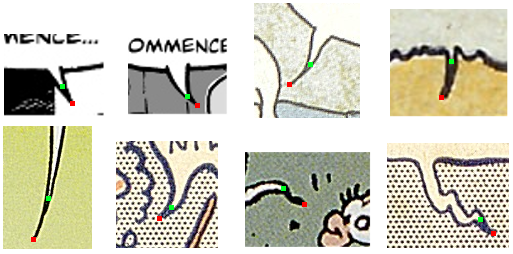
\includegraphics[width=0.9\textwidth]{tail_examples.png}
    \caption[Differences between tail tip positions]{Tail tip position differences considering the balloon background region or the balloon boundary. In each vignette, the green and red points represent the tail tip position from the balloon background or boundary point of view respectively.}
    \label{fig:se:tail_examples}
    \end{figure}
    %%%%%%%%%%%%%%%%%%%%%%%%%%%%%%%%%%%%%%%%%%%%%%%%%%%%%%%%

We propose to detect the tail position and direction based on the balloon contour analysis as tails are part of the balloon contour.
We limit this study to the tail types that can be considered has an extension of the inside region (background) of the speech balloon namely types ``comma'', ``zigzag'' and ``absent'' in Figure~\ref{fig:se:tail_types}, because they can all be extracted from the segmentation of the balloon background.
This limitation covers most of the speech balloons, nevertheless, other types such as ``stroke'' and ``circle'' in Figure~\ref{fig:se:tail_types}, require different approaches for speech balloon extraction (e.g. blob detection, contour boundary analysis).


% \paragraph{Tail tip position} % (fold)
% \label{par:se:tail_tip_position}

% paragraph tail_tip_position (end)

% We propose a method to detect ``comma'', ``zigzag'' and ``absent'' (no tail) tail types.
% The confidence value $C_{tail}$ may be useful for further decision making processes.
% If the speech balloon has no tail, there is no particular convexity defect.

The tail can be decomposed into four elements: origin, path, tip and pointed direction.
We call ``the origin'' the virtual point where the tail is plugged to the balloon.
The path is the symbolic line that represents the trajectory of the tail from the origin to its tip, we did not study this information in this work.
In contrast, the tail tip position is an important information because it is the anchor of the tail direction which indicate, when combined, the location of the speaking characters.
We propose a method based on convexity defects to detect the tail tip position and direction of ``comma'', ``zigzag'' and ``absent'' (no tail) tail types.
For each tail tip position detection, we compute a confidence value in order to be able to detect ``absent'' tails when the confidence is too low.
The directional angle of each tail is named with one direction corresponding to one of the eight cones of $\pi/4$ radians from the unit circle in order to facilitate further processing and evaluation (North, North Est, Est, South Est, South, South West, West and North West).

We observed that the contour of a speech balloon is mainly convex except in the region where the tail is plugged to the balloon (origin) which produces the highest convexity defects.
% and we can also detect it, see the end of this subsection.
%We propose to detect the two biggest convexity defects to locate the tail origin.
A convexity defect is defined by a triangle from one segment of the balloon convex hull to the farthest point on the balloon contour (Figure~\ref{fig:se:convexity_defects}).
The set $F=\{f_0,f_1,...f_n\}$ represents farthest points from the corresponding hull segments $S=\{s_0, s_1,...,s_n\}$ where $n$ is the number of hull segments.
We define the top two farthest points $f_a$ and $f_b$ corresponding to the two farthest points of the convex hull segments $s_a$ and $s_b$, as the coordinates of the tail origin (Figure~\ref{fig:se:convexity_defects}).

    %%%%%%%%%%%%%%%%%%%%%%%%%%%%%%%%%%%%%%%%%%%%%%%%%%%%%%%%
    \begin{figure}[ht]%trim=l b r t  width=0.5\textwidth,  
      \centering
      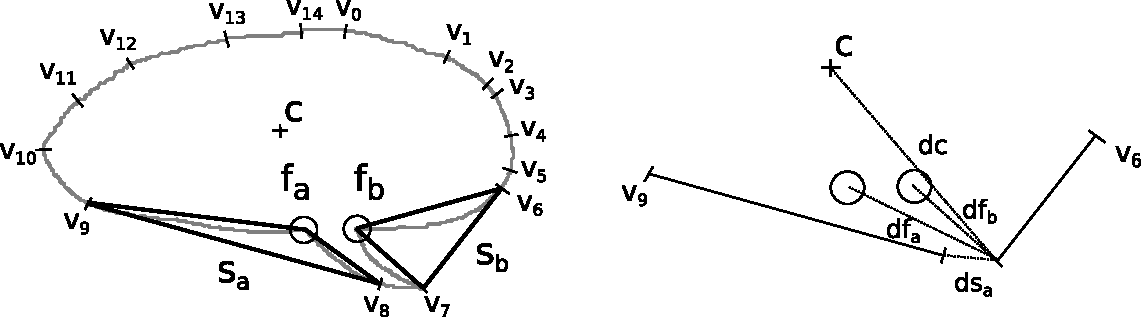
\includegraphics[width=0.9\textwidth]{tail_description.pdf}
    \caption[Convex hull and convexity defects of a speech balloon]{Convex hull and convexity defects of a speech balloon (top part). Bottom-left figure represents the two biggest convexity defects that defines the tail origin $f_a$ and $f_b$. Bottom-right figure represents the distances related to the vertex $v_7$ to illustrate the variables of Equation~\ref{eq:se:optimisation}. In this case $ds_b=0$ because $v_7$ coincides with an end of segment $s_b$ (distance equal to zero).}
    \label{fig:se:convexity_defects}
    \end{figure}
    %%%%%%%%%%%%%%%%%%%%%%%%%%%%%%%%%%%%%%%%%%%%%%%%%%%%%%%%

We assume that the tail tip corresponds to one of the vertices $V=\{v_0,v_1,...v_n\}$ of the convex hull (Figure~\ref{fig:se:convexity_defects}), which is the case for most of the speech balloons except when the tail is partially surrounded by the balloon (in a recess).
We did not consider such cases because they are uncommon and require a different approach.
The optimal vertex is computed by comparing five features that corresponds to the Euclidean distances:

\begin{itemize}
   \item $ds_a$ the distance to the segment $s_a$
   \item $ds_b$ the distance to the segment $s_b$
   \item $dc$ the distance to the centre of mass $c$ of the balloon
   \item $df_a$ the distance to the tail origin $f_a$
   \item $df_b$ the distance to the tail origin $f_b$
 \end{itemize}

This can be formulated as:
\begin{equation}\label{eq:se:optimisation}
   v* = argmax\big( max(dc+df_a+df_b) + min(ds_a + ds_b) \big)\\
 \end{equation}
 where $v*$ is the optimal vertex from the set of vertex $V$.
In Figure~\ref{fig:se:convexity_defects}, the optimal vertex is $v_7$.

%NEW IDEA: for all the vertex between the two defects, min/max a feature vector (dist to barycentre, distance to tail origin).
% Most of the time both triangles intersect on the same point which is the tail tip $T$.
% If not, we determine which pair of points from the two segments that are the closest ($t_1$ and $t_2$) and then which one is the tail tip ($t_1$ or $t_2$).
% The tail tip is defined by the farthest from the tail origin:
% $T = \begin{cases} t_1, & \mbox{if } dist(f_1,t_1) > dist(f_2,t_2) \\ t_2, & \mbox{else} \end{cases}$
%Each segment of the convect hull has a convexity defect that we $cd_i$

From our knowledge, all closed or implicit balloon extractors proposed so far, consider the inside balloon region and ignore the balloon contour (black stroke) region.
This is acceptable for localising the tail on the balloon contour (angular position) but it is not accurate enough to detect the tail tip in the sense of human understanding.
In fact, the tail tip is often located at the extremity of black stroke surrounding the inside balloon region (Figure~\ref{fig:se:tail_examples}).



We propose to detect the external border line of the balloon contour in the region of the optimal convex hull vertex $v*$ presented above and define its extremity as the tail tip position.
Image pre-processing and contour detection are performed in the same way as presented Section~\ref{sub:se:regular_balloon_extraction}.
From all the detected contours, we select the contour $O$ that has the closest point $o_i$ from $v*$ (Euclidean distance).
Then we run through all the points of the sequence of points that defines the contour $O=\{o_0, o_1,...,o_m\}$ and define as tail tip position $o*$ the one at the first maximum Euclidean distance to the tail origin.
The tail origin is a virtual point midway between $f_a$ and $f_b$ (Figure~\ref{fig:se:tail_tip_refinement}).

% \modif{TODO: update tail direction (improve) by computing a white region that includes the balloon border line}

The tail direction is given by the last part of the tail which corresponds to the vector $\overrightarrow{v*o*}$.
Note that starting from $v*$ is more accurate than the tail origin point because the last segment of the tail is oriented towards the speaker while the tail origin is just ``getting out'' of the balloon.


    %%%%%%%%%%%%%%%%%%%%%%%%%%%%%%%%%%%%%%%%%%%%%%%%%%%%%%%%
    \begin{figure}[ht]%trim=l b r t  width=0.5\textwidth,  
      \centering
      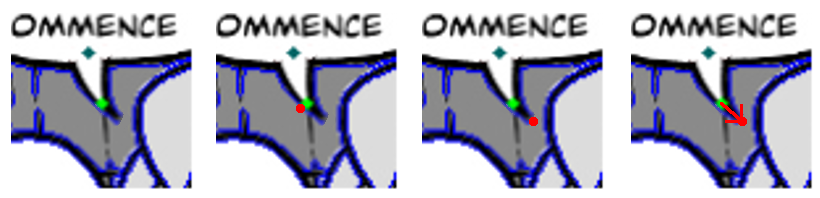
\includegraphics[width=0.95\textwidth]{tail_refinement.png}
    \caption[Tail tip position and direction detection]{Tail tip position and direction detection. From left to right, the optimal vertex $v*$ in green and the local contour detection in blue, the closest point to $v*$, $o_i$ in red and its first stop at the maximal distance with the tail origin (dark green point) $o*$. The last vignette on the right hand side represents the tail direction vector $\overrightarrow{v*,o*}$ by a white arrow.}
    \label{fig:se:tail_tip_refinement}
    \end{figure}
    %%%%%%%%%%%%%%%%%%%%%%%%%%%%%%%%%%%%%%%%%%%%%%%%%%%%%%%%

We also propose to compute the confidence value of the tail position prediction $C_{tail}$, related to the mean of the depths $d_a$ and $d_b$ over the mean balloon size $meanBalloonSize$ (Formula~\ref{eq:se:confidence_tail}).
The confidence value is minimal when the mean of the two convexity defects (used for tail position detection) is very small compared to the balloon sizes in the current image.
It is maximal when equal or higher than the mean balloon size.
% which means that the tail is at least as big as the balloons (clearly visible).

\begin{equation}
\label{eq:se:confidence_tail}
  C_{tail} = \frac{(d_a+d_b)/2}{meanBalloonSize}
\end{equation}
where $d_a$ and $d_b$ are the depth of the two biggest convexity defects in number of pixels (Figure~\ref{fig:se:convexity_defects}) and $meanBalloonSize$ is defined in equation~\ref{eq:se:mean_balloon_size}.

\begin{equation}
  \label{eq:se:mean_balloon_size}
  meanBalloonSize = \frac{\sum\limits_{i=0}^n W_{b_i} + \sum\limits_{i=0}^n H_{b_i}}{n * 2}  
\end{equation}
where $W_{b_i}$ and $H_{b_i}$ correspond to the width and the height of a speech  balloon $i$ and $n$ the number of speech balloons in the image.

% The confidence value $C_{tail}$ may be useful for further decision making processes.

% By measuring the variance in of all the convexity defect distances $\sum\limits_{i=0}^n var(f_i)$ of the contour we can detect if there is a tail or not, see equation~\ref{eq:se:var_defects}.
% We use a fixed threshold of $thV=10\%$ of the balloon height to decide if a balloon has a tail or not, see equation~\ref{eq:se:var_defects}.

% \begin{equation}
% \label{eq:se:var_defects}
%   hasTail = \begin{cases} 1, & \mbox{ if } \sum\limits_{i=0}^n var(f_i) > thV \\ 0, & \mbox{ else}  \end{cases}
% \end{equation}
% where $thV$ is a decision threshold relative to the average balloon size in the image.

% \paragraph{Tail direction} % (fold)
% \label{par:se:tail_direction}

% paragraph tail_direction (end)
% Once we found the tail tip position, we analyse its local region to find the orientation and the direction of the tail (directed towards the speaker).

% We compute a $M$x$M$ square region centred on the tail tip position in the balloon mask and use a line fitting algorithm (weighted least-squares) that returns the representative line that minimizes the distance between all the points of the local region (Figure~\ref{fig:se:orientation}).


%     %%%%%%%%%%%%%%%%%%%%%%%%%%%%%%%%%%%%%%%%%%%%%%%%%%%%%%%%
%     \begin{figure}[ht]%trim=l b r t  width=0.5\textwidth,  
%       \centering
%       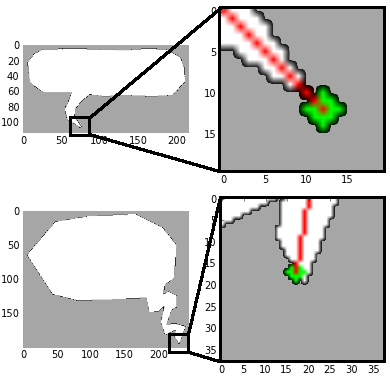
\includegraphics[width=0.5\textwidth]{tail_direction.png}
%     \caption[Tail orientation given by the line fitting algorithm in the neighbourhood of the tail tip]{Tail orientation given by the line fitting algorithm in the neighbourhood of the tail tip.}
%     \label{fig:se:orientation}
%     \end{figure}  
%    %%%%%%%%%%%%%%%%%%%%%%%%%%%%%%%%%%%%%%%%%%%%%%%%%%%%%%%%


% The tail direction is computed from the tail orientation that has initially two possible directions.
% We define the tail direction from the closest point $fitLinePoint$ of the representative line to the tail origin, to the tail tip ($vec\{fitLinePoint,$ $tailTip\}$).
 %by selecting the vector that starts close to the $F$ points and ends far from the $F$ points:

%$\dot{\vec{p}} = m\vec{v}$
% $\vec{vec\{dir\}} = \begin{cases} vec\{x_1,x_2\}, & \mbox{if } d(f_1,x_1) + d(f_2,x_1) < d(f_1,x_2) + d(f_2,x_2) \\ vec\{x_2,x_1\}, & \mbox{else} \end{cases}$

% section from_balloon_to_tail (end)


%--------------------------------------------------------------------------------------------------------------------------------------
\section{From tail to comic character} % (fold)
\label{sec:se:tail_to_character}


%from_tail_to_comic_character detecting the characters, in their great diversity, from the drawings of a comic book's page is quite a piece of work, 
% To detect comic characters from the tail detection, we narrow down the panel region according to position of the tail tip and to direction it is pointed to.
% area where we are going to look for them in.
% This can be done thanks to the panel, balloon and tail detection we extracted on the image during the previous steps.
% We make the assumption that the main characters of a story speak at some point.
% We focus on the characters that are emitting a speech balloon (speaking characters) and try to localize them from the speech balloon informations.
% That is to say that speech balloons will be associated one or several times to each of the character in different panels.

As presented Section~\ref{sec:sota:comic_character}, unsupervised comic character detection still an unsolved issue.
In fact, it faces tow difficulties.
The first one is the variety of comic styles that directly impacts the diversity of comic characters as they are the main elements of the stories (Figure~\ref{fig:kn:comics_diversity} and Appendix~\ref{sec:image_overview}).
The first challenge is to propose a generic approach able to cover such variety.
The second challenge is due to the variations of position, size, pose, scale, occluded parts between each instance of a given comic character (Figure~\ref{fig:sota:tarzan}).

Here we propose an approach that bypasses both issues by using already extracted information in order to predict the locations of the comic characters.
As we know which balloons are in which panel (total inclusion), we can estimate from the position and direction of the tail, which part of the panel may contain the speaking character.
This approach is limited to speaking characters but can be post processed in order to find non-speaking characters given the speaking ones as examples (Section~\ref{sub:complex_element_extraction}).

As mentioned in the previous section, the tail direction is quantized in eight cones of $\pi/4$ radius for simplification purposes so we can consider that, in a rectangular-shaped panel (or its bounding box), the tail is either pointing towards a corner or towards a border of the panel.
We define the ROI for the character as a squared region beside the speech balloon.
The maximum width $w_{max}$ and height $h_{max}$ of the ROI are equal to the mean widths and heights of all the balloons in the image (Equation \ref{eq:se:mean_balloon_size}).

The position of the ROI around the speech balloon is defined by two opposite points of a square $A_{x,y}$ and $B_{x,y}$ according to formula~\ref{eq:se:roi_position_around_balloon} which is sometimes constrained by a panel border that is why the term $min$ appears (Figure \ref{fig:se:roi_area}).
% The different positions of the ROI are illustrated on figure \ref{fig:se:roi_area}.

\begin{equation}
  \label{eq:se:roi_position_around_balloon}
  \begin{array}{rccl} 
	  A_x & = & v^*_x - min(Pi_x - v^*_x, w_{max}) & * O_x \\ 
	  A_y & = & v^*_y - min(Pi_y - v^*_y, h_{max}) & * O_y \\ 
	  B_x & = & \left[ A_x + min(Pi_x - A_x, w_{max}) \right] & * O_x \\ 
	  B_y & = & \left[ A_y + min(Pi_y - A_y, h_{max}) \right] & * O_y
  \end{array} 
\end{equation}
where $v^*$ is the coordinates of the tail tip (Section~\ref{sec:se:from_balloon_to_tail}), $Pi$ the coordinates of one of the four corners of the panel bounding box $P=\{P0, P1, P2, P3\}$ and $O$ a shift value.
The shift value allows an horizontal and vertical translation of the ROI position relatively to the tail tip direction (Figure~\ref{fig:se:roi_area}).
% For instance, if the tail direction is SE (South Est) the ROI will be shifted by 75\% on the right and 75\% to the bottom.
The shift $O$ is quantized in heigh values, according to the tail direction quantization (Section~\ref{sec:se:from_balloon_to_tail}), for horizontal and vertical axis.
The panel's corner $P_i$ is chosen between two opposite corners in order to always give a positive value in the computation of the ROI position (Table~\ref{tab:se:offset_panel_corner}).

    %%%%%%%%%%%%%%%%%%%%%%%%%%%%%%%%%%%%%%%%%%%%%%%%%%%
  \begin{table}[ht]
    \normalsize
%\renewcommand{\arraystretch}{1.2}

    \centering
    \caption{Values of the horizontal and vertical shifts and panel's corner selection according to the eight directions of the tail.}
    % \def\arraystretch{1.5}%  1 is the default, change whatever you need
    \setlength{\tabcolsep}{.45em}
    % \extracolsep{\fill}
    \begin{tabular}{|c|c|c|c|c|c|c|c|c|}

          \hline
	      &  N  & NE  & E  & SE & S & SW & W & NW   \\
	      \hline
	      $O_x$   & 0.5  & 0.75 & 1.0  & 0.75 & 0.5 & -0.75& -0.5 & 0.75  \\
	      \hline
	      $O_y$   & -1   & -0.75& -0.5 & 0.75 & 1.0 & 0.75 & -0.5 & -0.75  \\
	      \hline
	      $Pi$    & P1   & P1   & P1   & P1   & P3  & P3   & P3   & P3   \\
          \hline
        \end{tabular}
    \label{tab:se:offset_panel_corner}
  \end{table}%
    %%%%%%%%%%%%%%%%%%%%%%%%%%%%%%%%%%%%%%%%%%%%%%%%%%%


% Sometimes the pointed corner or border is far from the tail tip and create a wide region.

%An analysis of the eBDtheque ground truth gave us the confirmation that this estimated areas were actually containing more than 70\% of the characters with a precision of 50\% in average.

%%%%%%%%%%%%%%%%%%%%%%%%%%%%%%%%%%%%%%%%%%%%%%%%%%%
 \begin{figure}[!ht]
   \centering
  %\includegraphics[width=150px]{fig/roi_area.pdf}
  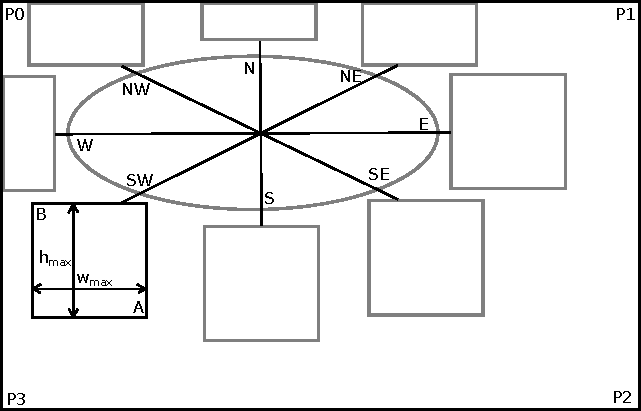
\includegraphics[width=180px]{roi_hypothesis.pdf}
  \caption[Illustration of the character region of interested computation for each of the eight directions of the tail]{Illustration of a panel with four corners $P0, P1, P2, P3$ and the different ROI position and size that can be defined for each of the eight directions of the tail.
  }
  \label{fig:se:roi_area}
 \end{figure}
%%%%%%%%%%%%%%%%%%%%%%%%%%%%%%%%%%%%%%%%%%%%%%%%%%%

% The ROI are then passed to the comic character extractor (see section~\ref{sub:character_extraction}) which will locate more precisely the characters based on image features.
% image processing part (character extractor) that will spot all the characters, especially the ones that does not speak, using those regions as seeds.


% section from_tail_to_comic_character (end)

% Conclusion --------------------------------------------------------------------------------------------------------------------------------------
\section{Conclusions}
\label{sec:se:conclusion}
In this section we have presented how to benefit from simple element to retrieve more complex ones in a comics image by following the relations between elements.
This approach is similar to the reader's reading behaviour opening a new comic book for the first time: first looking for traditional elements such as the panels, text and speech balloons and then, reading their content and retrieving the links with the comic characters and other graphics in the panel.
This first approach is driven by the image content which means that each newly extracted element allows other related elements to be retrieved.
% The domain knowledge is embedded into each specific extraction algorithms.
It is particularly useful for ensuring a certain consistency between all the extracted elements but in return, the dependency of the processes propagates extraction errors.
For instance, if a panel is not extracted then its content will not be processed and potential balloons and comic characters will be missed.
% Despite the intuitiveness of this approach
The experiments, presented in \ch{chap:experimentations}, evaluate and compare this approach to methods from the literature and other approaches that will be presented in the two next chapters.

% In this section we have presented and evaluated two methods for panel extraction based on connected-components labelling.
% The experiments shows that both approaches are really efficient for comics using gutter where there is no drawing between panels.
% The first method have been published for national and international audience~\cite{rigaud2012extraction,Rigaud2012LNCS} and the second method is part of an international journal publication [pending acceptance???].

% Then, the variance of each class is computed to check the homogeneity of the ROI. If the variance of the ``frame'' class is high, a specific algorithm~\cite{Khoi11} is applied in order to improve the previous steps (binarisation and/or classification). 

In the next chapter a non-sequential approach will be presented in order to extract comics image content using independent processing and so, avoid error propagation which is the main drawback of applying several consecutive processing.

% Also, an open balloon detection method based on speech text position will be presented.


% \begin{itemize}
% 	% \item Compute a confidence value between 0 and 1 for each panel: the inverse of overlapping percentage with other panels. (maximal when no overlap). This can replace the topological filtering by considering as correct the panel with a confidence > 0\%
% 	\item \url{/PhD/publication/2013/LNCS/robust_frame_and_text_extraction_from_comic_books/paper}
% 	\item IJDAR paper > panel extraction %\url{/PhD/Publications/CIFED_2012}
% \end{itemize}
